\documentclass[12pt]{article}
\usepackage[margin=2cm, bindingoffset=0cm]{geometry}
%\usepackage[german]{babel} 
\usepackage[ngerman]{babel} %sudo apt-get install texlive-lang-german
\usepackage{hyperref} % web links etc.
\usepackage[parfill]{parskip}
\usepackage[utf8]{inputenc}
\usepackage[dvipsnames]{xcolor}
\usepackage{tcolorbox}
\usepackage{helvet} 
\usepackage{framed}
\usepackage{anyfontsize}
\usepackage{csquotes}
\usepackage{mathrsfs}
\usepackage{physics}
\setcounter{MaxMatrixCols}{16}
\usepackage{amssymb}
\usepackage{MnSymbol}
\MakeOuterQuote{"}
\definecolor{quotecolor}{rgb}{0.8,0.9,1}
\renewcommand{\familydefault}{\sfdefault} 
\setlength\parindent{0pt}
\tcbset{boxrule=0pt,colback=quotecolor,arc=5pt,auto outer arc,left=5pt,right=5pt,boxsep=5pt}
%  width=0.9\textwidth,

\setcounter{secnumdepth}{-1}
\begin{document}
\title{\fontsize{25}{25}\selectfont \textbf{Über psychische und physikalische Zeit}}
\author{Harald Rieder}
\date{\today}
\maketitle

%\begin{abstract}

%\end{abstract}

\tableofcontents

\section{Motivation}

Der Erfolg der relativistischen Physik lehrt uns, dass die Zeit irgendwie gleichrangig neben dem Ort zu stehen hat. Wechselt ein Beobachter seine Perspektive auf bestimmte Art, sehen  Koordinaten, die zuvor wie reine Ortskoordinaten ausgesehen haben, plötzlich ein wenig wie Zeitkoordinaten aus, und umgekehrt. Ein solcher Perspektiv-Wechsel heißt in der speziellen Relativitätstheorie \emph{Lorentz-Transformation}.\footnote{Ein Beispiel aus der allgemeinen Relativitätstheorie: Beim Passieren des Ereignishorizontes der Schwarzschild-Metrik tauschen Radialterm und Zeitterm ihre Vorzeichen aus. Nach dem starken Äquivalenzprinzip ist so ein Standortwechsel lokal äquivalent zu einem Wechsel der Perspektive.} 

Der Alltag lehrt uns, dass die Zeit kontinuierlich vergeht, und zwar in eine bestimmte Richtung. Denn das Alltagsgeschehen scheint sich meistens nicht umkehren zu lassen. Eine zerschellte Tasse setzt sich nicht mit der Zeit wieder zu einer heilen Tasse zusammen und kehrt unter Abkühlung auf den Tisch zurück. Solches Alltagsgeschehen wird durch den 2. Hauptsatz der Thermodynamik erfolgreich modelliert.

Der Erfolg der Physik insgesamt lehrt uns, dass Ortsraum keine eingebaute Richtung hat. Es gibt keinen Satz der behauptet, dass wenn man in eine bestimmte Richtung geht, die Tassen immer kaputter werden müssen.

Somit haben wir 3 erfolgreich anwendbare Konzepte, die im Widerspruch zu stehen scheinen. Raum und Zeit sind wie Bruder und Schwester. Die Zeit hat eine eingebaute Richtung, der Raum aber nicht. Und nun?

Darum schauen wir uns an, wozu uns ein paar unkonventionelle Annahmen führen können:

\begin{itemize}
\item In der Physik vergeht keine Zeit. Die Natur der physikalischen Zeit ist wie die Natur des physikalischen Ortsraums.
\item In der Psyche vergeht Zeit. Sie ist integraler Bestandteil des Bewusstwerdens, des Geistes. 
\item Es muss einen Mechanismus geben, der die psychische Zeit mit einem Bestandteil der physikalischen Welt so koppelt, dass es wenigstens für die menschliche Psyche den Anschein hat, die physikalische Zeit würde objektiv vergehen.
\end{itemize}

\section{Idee zu einer Quantenuhr}

In der Quantenmechanik spielt sich das Geschehen in einem vieldimensionalen Konfigurationsraum ab, dem Hilbert-Raum. Ein Ort existiert in diesem Raum zunächst nicht. Erst durch Festlegung auf eine Basis lassen sich komplexwertige Funktionen erstellen. Diese Funktionen stehen für unendlich viele Amplituden, die durch einen kontinuierlichen reellwertigen Index $x$ durchnummeriert werden.

Durch Beobachtung von außen, sowie durch Symmetrien, die wir aus der Erfahrung her einem dreidimensionalen Ortsraum zuschreiben, gelingt uns der Anschluss. Es sind unendlich viele Basen wählbar, doch nur bestimmte Wahlen führen zu einer Indexierung, bei der wir den Index als Ortskoordinate interpretieren können. Die Amplitude eines abstrakten Zustandsvektors $\ket{\psi}$ an einem bestimmten Ort liefert uns das Skalarprodukt mit dem abstrakten Vektor einer "Ortsbasis"
\begin{equation} 
\psi(x) \equiv \bra{x}\ket{\psi} 
\end{equation}
Wenn wir die physikalische Zeit ähnlich wie den Ort behandeln wollen, dann muss die Zeitkoordinate $t$ ebenso ein reellwertiger kontinuierlicher Index sein. Das heißt
\begin{equation} 
\label{eq:psi_xt}
\psi(t,x) \equiv \bra{t,x}\ket{\psi} 
\end{equation}
Die Indizes $x$ und $t$ nummerieren nun zusammen eine Produktbasis aus Orts- und Zeiteigenvektoren. Wir könnten aufgrund der Gleichmächtigkeit von $\mathbb{R}$ mit $\mathbb{R}^2$ diesen Index durch einen gemeinsamen reellwertigen Index $s = s(x,t)$ ersetzen und kämen damit wieder auf die Form
\begin{equation}
\label{eq:psi_s}
\psi(s) \equiv \bra{s}\ket{\psi} 
\end{equation}
wobei $\ket{\psi}$ wie in (\ref{eq:psi_xt}) der abstrakte Zustandsvektor im Produktraum wäre.

Wir nehmen an, dass der Beobachter aus seinem Hilbert-Raum $\mathscr{H}_X$ heraus nicht in der Lage dazu ist, Zeit "direkt" in Erfahrung zu bringen. Diese Annahme drückt sich in der Quantenmechanik so aus, dass in Matrixelementen $H(X,x)$ von Wechselwirkungs-Hamiltonians die Zeit nicht auftritt. Ein Beobachter muss eine Zeigerstellung, einen Ort, ablesen, um von dort auf die Zeit im Uhrenzustand zu schließen. 

\begin{figure}[!h]\begin{center}
  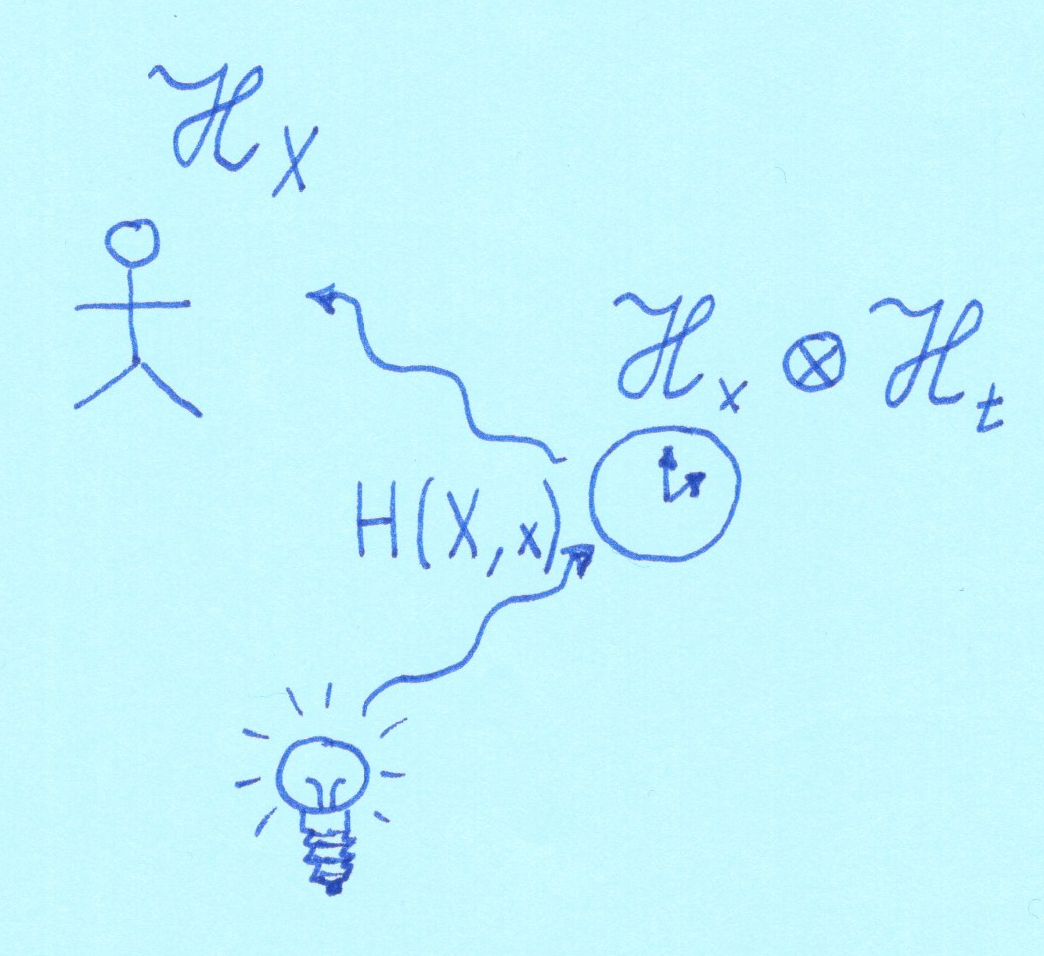
\includegraphics[width=6cm]{Quantenuhr.png}
  \caption{Indirektes Ablesen der Uhrzeit}
  \label{fig:clock}
\end{center}\end{figure}

Ein guter Uhrenzustand kann also ein Zustandsvektor im Produktraum $\mathscr{H}_x \otimes \mathscr{H}_t$ sein, der Orts- und Zeitunterräume maximal verschränkt. Wenn $\delta(x-\xi)$ die Amplituden von Ortseigenvektoren im Ortsunterraum in der Ortsdarstellung sind, und $\delta(t-\tau)$ die Amplituden von Zeiteigenvektoren im Zeitunterraum in der Zeitdarstellung, dann sind\footnote{Fortan lassen wir die Integralgrenzen weg, wenn sie im Unendlichen liegen.}
\begin{equation} 
\label{eq:psi_clock}
\psi(t,x) \sim \int_{-\infty}^{\infty} \mathrm d\chi \, \delta(t-\chi) \delta(x-\chi) = \delta(t-x)
\end{equation}
die Amplituden eines maximal verschränkten Zustands, der aus der Beobachtung von $\xi$ sicher auf die Zeit $\tau$ schließen lässt. Durch die Beobachtung (oder Messung) "kollabiert die Überlagerung"
\begin{equation} 
\label{eq:collapse}
\int \mathrm d\chi \, \delta(t-\chi) \delta(x-\chi) \quad \rightarrow \quad \delta(t-\chi)\delta(x-\chi)
\end{equation}
Dadurch ist die Uhr zunächst kaputtgegangen. Denn durch verträgliche Messungen, also wiederholte Ortsmessungen, werden wir immer wieder nur diesen Zustand und damit die Zeit $\chi$ antreffen. Es fehlt also ein Mechanismus, der die Uhr wieder scharfschaltet, sie in ihren verschränkten Zustand zurückbringt.

Im Artikel \emph{\href{https://docs.google.com/document/d/1OrmVETmnBSe5c0CpTbKH8Vq5pWFuB8QUez-KqHTaarQ/edit?usp=sharing}{Ideas about a Quantum Theory without Process Type 2}} wird so ein Mechanismus vorgestellt. Dort wird postuliert, dass jeder bewusste Beobachter einerseits eine Teilung des Hilbertraums vornimmt, andererseits die Änderung der Verschränkungen, wie sie erst durch die jeweilige Teilung aus den jeweils vorliegenden Zustandsvektoren entstehen, erlebt, ja sie womöglich willentlich herbeiführen kann, wodurch dann \emph{aus Sicht des jeweiligen Beobachters} die quantenmechanische Überlagerung kollabiert und am Ende ein reiner Produktzustand vorliegt. Mindestens 2 solcherart an den physikalischen Kanal angeschlossene Beobachter (\emph{conscious splits}) sind notwendig, um ein Geschehen am Laufen zu halten. Unsere Uhr soll von einem äußeren Beobachter wie gezeigt hin und wieder abgelesen werden. Wir benötigen also noch einen weiteren "internen" Beobachter, der den x,t-Produktraum auf andere Weise teilen muss als der externe Beobachter. Der interne Beobachter teilt den Produktraum dazu nicht in x- und t-Basen, sondern in eine Basis aus x,t-verschränkten Zuständen und eine Basis, die den ganzen Rest enthält.

Um zu sehen, wie es läuft, betrachten wir ein einfaches Beispiel...

\section{Eine Quantenuhr aus 2 Qutrits}

Unsere einfache Quantenuhr soll nur 3 diskrete Zeigerstellungen haben: $\ket{x=0}, \ket{x=1}, \ket{x=2}$. Sie soll auch nur 3 Zeitpunkte messen können: $\ket{t=0}, \ket{t=1}, \ket{t=2}$. Wir lassen später der Übersichtlichkeit halber x und t weg, x soll links stehen, t rechts. Das heißt zum Beispiel $\ket{00}$ soll für $\ket{x=0}\ket{t=0}$ stehen. 

Wir haben es mit einem Produktraum aus 2 Qutrits, 1 Raum- und 1 Zeit-Qutrit zu tun. Für eine Orthogonalbasis sind somit 9 Basisvektoren notwendig. Wir bilden diese aus den Produkten der 3 Raum- und 3 Zeit-Eigenvektoren.

Einen x,t-verschränkten Zustand können wir zum Beispiel so bilden
\begin{equation*}
\frac{1}{\sqrt{2}} \left(\, \ket{x=0}\otimes\ket{t=0} + \ket{x=1}\otimes\ket{t=1} \,\right) \equiv 
\frac{1}{\sqrt{2}} \left(\, \ket{00} + \ket{11} \,\right)
\quad\quad\hat{=}\quad\quad
\frac{1}{\sqrt{2}}
\begin{pmatrix}
1 \\ 0 \\ 0 \\ 0 \\ 1 \\ 0 \\ 0 \\ 0 \\ 0 
\end{pmatrix}
\quad
\begin{matrix}
00 \\ 01 \\ 02 \\ 10 \\ 11 \\ 12 \\ 20 \\ 21 \\ 22 
\end{matrix}
\end{equation*}
und einen unverschränkten Zustand so
\begin{equation*}
\frac{1}{\sqrt{2}}\, \ket{x=1}\otimes \left(\,\ket{t=0} + \ket{t=2} \,\right) \equiv 
\frac{1}{\sqrt{2}} \left(\, \ket{10} + \ket{12} \,\right)
\quad\quad\hat{=}\quad\quad
\frac{1}{\sqrt{2}}
\begin{pmatrix}
0 \\ 0 \\ 0 \\ 1 \\ 0 \\ 1 \\ 0 \\ 0 \\ 0 
\end{pmatrix}
\quad
\begin{matrix}
00 \\ 01 \\ 02 \\ 10 \\ 11 \\ 12 \\ 20 \\ 21 \\ 22 
\end{matrix}
\end{equation*}
Dies ist die Perspektive des äußeren Beobachters. Die Uhr soll ihm verschränkte Zustände anbieten, die aus Linearkombinationen von $\ket{\chi\chi}$ Vektoren zusammengesetzt sind. Er entscheidet sich dann für einen der Vektoren mit einer Wahrscheinlichkeit gemäß der Bornschen Regel. 

Daraufhin muss die Uhr wieder scharfgeschaltet werden, wozu wir den internen Beobachter brauchen. Für den internen Beobachter müssen alle $\ket{\chi\chi}_{ext}$ Zustände verschränkt aussehen, damit er tätig wird. Um auf seine Perspektive zu wechseln, brauchen wir eine unitäre Matrix $U$ im Produktraum, zum Beispiel\footnote{Elemente mit Wert 0 lassen wir der Übersichtlichkeit halber nun öfter weg.}
\begin{equation}
U\ =\ 
\begin{pmatrix}
\label{eq:U}
\pmb{a_0} &&&&& \pmb{a_2} &&&&& \pmb{a_1} \\
  & 1 &   &   &   &   &   &   &   &   &   \\
  &   & 1 &   &   &   &   &   &   &   &   \\
  &   &   & 1 &   &   &   &   &   &   &   \\
\pmb{a_1} &&&&& \pmb{a_0} &&&&& \pmb{a_2} \\
  &   &   &   &   &   & 1 &   &   &   &   \\
  &   &   &   &   &   &   & 1 &   &   &   \\
  &   &   &   &   &   &   &   & 1 &   &   \\
\pmb{a_2} &&&&& \pmb{a_1} &&&&& \pmb{a_0} \\
\end{pmatrix}
\quad
\begin{matrix}
00 \\ 01 \\ 02 \\ 10 \\ 11 \\ 12 \\ 20 \\ 21 \\ 22 
\end{matrix}
\end{equation}
Die komplexen Werte $a_0$, $a_1$, $a_2$ an den Stellen, die für x,t-Verschränkung stehen, rotieren ihre Plätze in den 3 betroffenen Spaltenvektoren und ebenfalls in den betroffenen Zeilenvektoren. Die Werte sind geeignet zu wählen, worauf wir noch kommen werden.

Hat der externe Beobachter zum Beispiel die Zeit t=0 gemessen, dann ist die Uhr im Zustand $\ket{00}_{ext}$. Dieser Zustand ist aus Sicht des internen Beobachters eine Verschränkung aus $\ket{00}_{int}$, $\ket{11}_{int}$ und $\ket{22}_{int}$.\footnote{Welche Bedeutung für ihn die Ziffernpaare haben, wissen wir nicht.} Mit den Bornschen Wahrscheinlichkeiten kollabiert die Überlagerung aus seiner Sicht:
\begin{equation*}
\begin{matrix}
\ket{00}_{ext} \ \xrightarrow{U} \ a_0\ket{00}_{int} + a_1\ket{11}_{int} + a_2\ket{22}_{int} 
& \xrightarrow{p = |a_0|^2} & \ket{00}_{int} \\ \\
& \xrightarrow{p = |a_1|^2} & \ket{11}_{int} \\ \\
& \xrightarrow{p = |a_2|^2} & \ket{22}_{int}
\end{matrix}
\end{equation*}
Damit das Geschehen weiterläuft, benötigen wir wieder den externen Beobachter. Die Inverse von $U$ transformiert zurück auf dessen Sicht und lässt unverschränkte interne Zustände $\ket{\chi\chi}_{int}$ verschränkt erscheinen.
\begin{equation}
U^{-1}\ =\ 
\begin{pmatrix}
\label{eq:not_U}
\pmb{a_0} &&&&& \pmb{a_1} &&&&& \pmb{a_2} \\
  & 1 &   &   &   &   &   &   &   &   &   \\
  &   & 1 &   &   &   &   &   &   &   &   \\
  &   &   & 1 &   &   &   &   &   &   &   \\
\pmb{a_2} &&&&& \pmb{a_0} &&&&& \pmb{a_1} \\
  &   &   &   &   &   & 1 &   &   &   &   \\
  &   &   &   &   &   &   & 1 &   &   &   \\
  &   &   &   &   &   &   &   & 1 &   &   \\
\pmb{a_1} &&&&& \pmb{a_2} &&&&& \pmb{a_0} \\
\end{pmatrix}
\quad
\begin{matrix}
00 \\ 01 \\ 02 \\ 10 \\ 11 \\ 12 \\ 20 \\ 21 \\ 22 
\end{matrix}
\end{equation}
Insgesamt haben wir nun einen stochastischen Prozess vorliegen. Die absolutquadrierten Elemente von $U$ und $U^{-1}$ liefern uns die Wahrscheinlichkeiten für Zustandsübergänge. Nur die fettgedruckten Elemente in (\ref{eq:U}) und (\ref{eq:not_U}) tragen zum Geschehen bei, wenn wir mit $\ket{\chi\chi}_{ext}$ Zuständen starten. Wir können die anderen Elemente somit weglassen und bekommen übersichtlichere 3x3-Matrizen. Wenn wir interne und externe Sicht noch in einem 6-komponentigen Vektor zusammenfassen, können wir eine \emph{unistochastische} Matrix $P$ angeben, die den Prozess beschreibt und von Bornschen Wahrscheinlichkeiten bevölkert ist.
\begin{equation}
P\, =\,
\begin{pmatrix}
0 & \{|U_{ji}|^2\} \\
\{|U_{ij}|^2\} & 0
\end{pmatrix}
\end{equation}
In unserem Beispiel ist die stochastische Matrix, wenn wir noch $|a_i|^2$ durch $p_i$ abkürzen
\begin{equation}
P\, =\,
\begin{pmatrix}
&&& p_0 & p_1 & p_2 \\
&&& p_2 & p_0 & p_1 \\
&&& p_1 & p_2 & p_0 \\
p_0 & p_2 & p_1 &&& \\
p_1 & p_0 & p_2 &&& \\
p_2 & p_1 & p_0 &&& 
\end{pmatrix}
\quad
\begin{matrix}
00_{ext} \\ 11_{ext} \\ 22_{ext} \\ 00_{int} \\ 11_{int} \\ 22_{int}
\end{matrix}
\end{equation}
Das Quadrat der Matrix $P$, also $Q:=P^2$, bedeutet einen Wechsel auf die interne Sicht und wieder zurück. Es steht sozusagen für einen Tick der Zeit und liefert die Wahrscheinlichkeiten, mit denen der externe Beobachter einen bestimmten x,t-verschränkten Zustand nach dem Tick beobachtet in Abhängigkeit des Zustands vor dem Tick.

Wir wählen nun konkrete Zahlenwerte für die Uhr. Im Anhang wird gezeigt, wie man auf geeignete Werte kommt.
\begin{equation*}
a_0=N\frac{sin(\alpha_0+\alpha_1)}{sin(\alpha_1-2\alpha_0)}e^{i\alpha_0} \quad
a_1=N\frac{sin(\alpha_0+\alpha_1)}{sin(\alpha_0-2\alpha_1)}e^{i\alpha_1} \quad
a_2=N
\end{equation*}
mit 
\begin{equation*}
N\, = \, \left( 1 +
\frac{sin^2(\alpha_0+\alpha_1)}{sin^2(\alpha_1-2\alpha_0)} +
\frac{sin^2(\alpha_0+\alpha_1)}{sin^2(\alpha_0-2\alpha_1)} \right)^{-\frac{1}{2}}
\end{equation*}
Und wir wählen die Winkel zu
\begin{equation*}
\alpha_0 = \pi / 6 \quad \alpha_1 = \pi / 5 \\ \\
\end{equation*}
Damit werden 
\begin{equation*}
P\, \approx\,
\begin{pmatrix}
   &&& 0.63787 &  0.12644 &  0.23569 \\
   &&& 0.23569 &  0.63787 &  0.12644 \\
   &&& 0.12644 &  0.23569 &  0.63787 \\
   0.63787 &  0.12644 &  0.23569 &&& \\
   0.23569 &  0.63787 &  0.12644 &&& \\
   0.12644 &  0.23569 &  0.63787 &&& 
\end{pmatrix}
\quad
\begin{matrix}
00_{ext} \\ 11_{ext} \\ 22_{ext} \\ 00_{int} \\ 11_{int} \\ 22_{int}
\end{matrix}
\end{equation*}
und
\begin{equation*}
Q=P^2\, \approx\,
\begin{pmatrix}
   0.47841 & 0.26079 & 0.26079 &&& \\
   0.26079 & 0.47841 & 0.26079 &&& \\
   0.26079 & 0.26079 & 0.47841 &&& \\
   &&& 0.47841 & 0.26079 & 0.26079 \\
   &&& 0.26079 & 0.47841 & 0.26079 \\
   &&& 0.26079 & 0.26079 & 0.47841
\end{pmatrix}
\quad
\begin{matrix}
00_{ext} \\ 11_{ext} \\ 22_{ext} \\ 00_{int} \\ 11_{int} \\ 22_{int}
\end{matrix}
\end{equation*}
Erwartungswerte für die beobachtete Zeit können wir so bilden
\begin{equation*}
<t> = t \cdot Q \cdot \psi \quad\quad t = \begin{pmatrix}
0&1&2&0&0&0
\end{pmatrix}
\end{equation*}
In unserem Beispiel ergeben sich in Abhängigkeit des Ausgangszustands die Erwartungswerte
\begin{center}
\begin{tabular}{ |c|c| } 
 \hline
 $\psi$ & $<t>$ \\ 
 \hline
 $\ket{00}_{ext}$ & 0.78 \\ 
 $\ket{11}_{ext}$ & 1.00 \\ 
 $\ket{22}_{ext}$ & 1.22 \\
 \hline
\end{tabular}
\end{center}
Eine makroskopische Uhr, die über viele Quantenuhren mittelt, würde uns diese Zeitwerte liefern. Ausgehend von t=0 liefe die gemessene Zeit also vorwärts, bei t=1 bliebe sie stehen, ausgehend von t=2 liefe sie rückwärts. Könnten wir mit sehr großen Matrizen $U$ hantieren, dann könnten wir womöglich große Bereiche schaffen, in denen die Zeit vorwärts liefe und solche, in denen sie rückwärts liefe. In jedem solchen Bereich erführe der externe Beobachter aber \emph{im Mittel eine in eine bestimmte Richtung laufende Zeit}.

Größere doppelt-stochastische Matrizen mögen sich zu diesem Zweck noch leicht zurechtlegen lassen. Allerdings ist die Frage, ob sie auch unistochastisch sind, ab einer Zeilenzahl von 5 und dem heutigen Stand der Forschung leider kaum beantwortbar. Unistochastisch müssen sie aber sein, wenn sie mit der Quantenmechanik verträglich sein sollen.

\section{Wachsen der Entropie mit der psychischen Zeit}

Doppelt-stochastische Übergangsmatrizen in Markov-Prozessen führen im Limes zu einer Gleichverteilung der Wahrscheinlichkeiten. Doch was bedeutet das in unserem Zusammenhang?

%The stationary distribution of an irreducible aperiodic finite Markov chain is uniform if and only if its transition matrix is doubly stochastic.

Wir nehmen an, dass eine Beobachterin A im Hilbert-Raum $\mathscr{H}_Y$ das System der Abbildung \ref{fig:clock} sozusagen von ganz außen beobachtet. 
\begin{figure}[!h]\begin{center}
  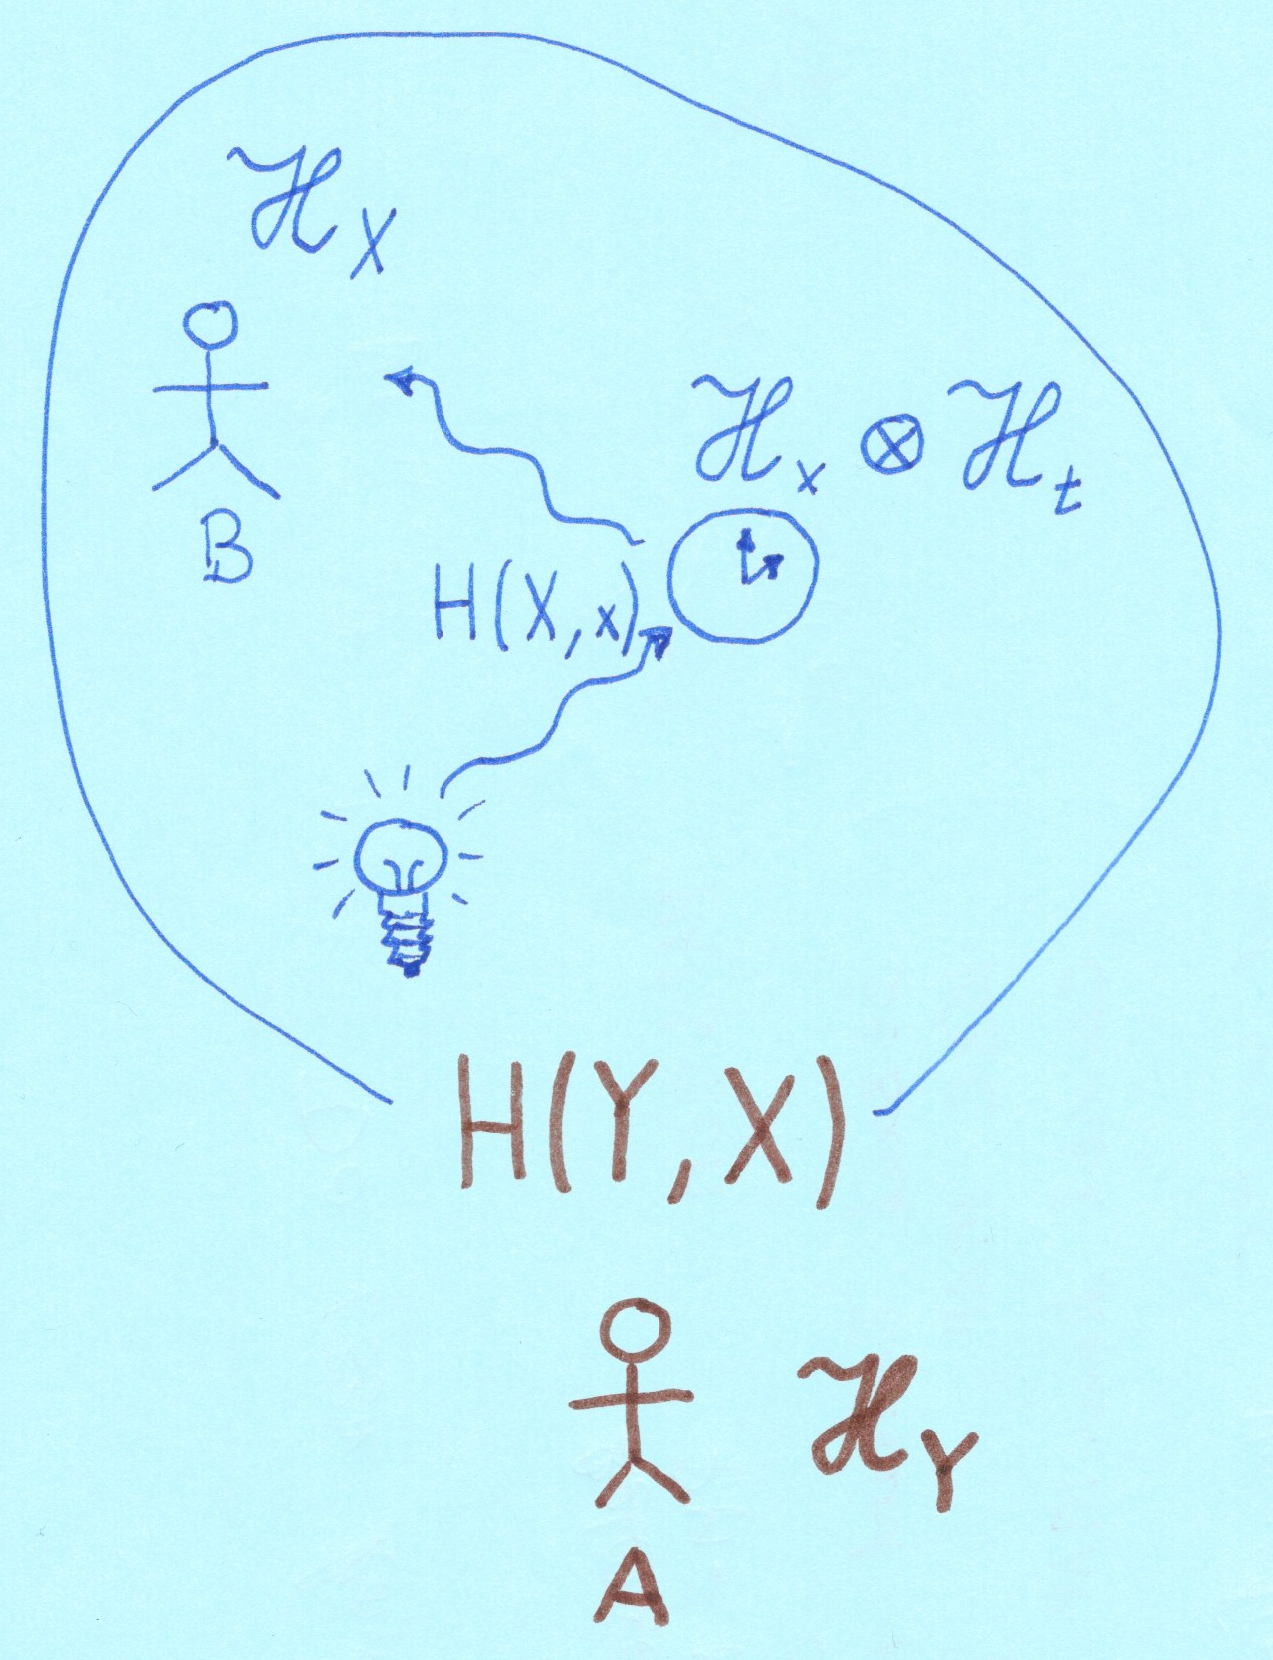
\includegraphics[width=6cm]{Entropie.png}
  \caption{Ganz äußere Beobachterin}
  \label{fig:entropy}
\end{center}\end{figure}
Die Beobachterin wechselwirkt mit ihren eigenen Uhren und erlebt dadurch ein Fortschreiten ihrer Zeit. Von Zeit zu Zeit koppelt sie sich mit einem Wechselwirkungs-Hamiltonian $H(Y,X)$ an den Beobachter B, um ihn nach seiner Zeit zu fragen. Wenn B antwortet, dass er $\chi$ gemessen habe, dann weiß sie, dass das System im Zustand 
\begin{equation}
\ket{X=\chi}\otimes\ket{\chi\chi}
\end{equation}
ist - oder gerade noch gewesen ist. Die Abfrage der Zeit von B durch A ist natürlich auch ein Quantenprozess. Wir können ihn uns als Dekohärenz-Prozess im Grenzfall einer Quantenmessung vorstellen. Das heißt, wenn B "das Wissen $\chi$" erlangt hat, soll im Idealfall der Gesamtzustand
\begin{equation}
\ket{\Theta}\ \ =\ \ \ket{Y=\chi}\otimes\ket{X=\chi}\otimes\ket{\chi\chi}
\end{equation}
vorliegen.\footnote{Bei makroskopischen Beobachtern müssen wir uns die Unterräume von $\mathscr{H}_Y$ und $\mathscr{H}_X$ zum Messwert $\chi$ stark entartet denken.}  Dieser reine Zustand hat die Entropie 0. Formal können wir den Dichteoperator $\hat{\rho}$ des Systems durch Ausspuren der Freiheitsgrade von Y bilden
\begin{equation}
\hat{\rho}_{\chi,\chi\chi}\ =\ \operatorname{Spur}_Y \ket{\Theta}\bra{\Theta}\ =\ 
\ket{X=\chi}\otimes\ket{\chi\chi}\ \bra{\chi\chi}\otimes\bra{X=\chi} 
\end{equation}
und erhalten für dessen von-Neumann-Entropie
\begin{equation}
S\ =\ -\operatorname{Spur} \hat{\rho}_{\chi,\chi\chi} \log_2\ \hat{\rho}_{\chi,\chi\chi}\ = \ 0
\end{equation}
Bis zur nächsten Abfrage sollen $\tau$ Ticks im System vergehen. Die Matrix $Q$ wirkt bei jedem Tick, so dass nach $\tau$ Ticks die Wahrscheinlichkeiten für die Endzustände
\begin{equation}
p_i=\sum_j \{Q^\tau\}_{ij}\, \delta_{j\chi}
\end{equation}
sind. Nun haben wir aus Sicht von B ein Gemisch im System vorliegen
\begin{equation}
\hat{\rho}_{X,xt}\ = \ \sum_{i=0}^{n-1} p_i \ket{X=i}\otimes\ket{ii}\ \bra{ii}\otimes\bra{X=i} 
\end{equation}
$n$ soll für die endliche Mächtigkeit des Hilbertraums des Systems stehen. Im Limes $\tau\rightarrow\infty$ streben die $p_i$ nach demselben Wert $p_\infty=n^{-1}$, was die Maximierung der von-Neumann-Entropie des Systems bedeutet. Mit den Matrixelementen von $\hat{\rho}_{X,xt}$ ausgedrückt
\begin{equation}
S_\infty\ =\ -\operatorname{Spur} \left(
\begin{pmatrix}
p_\infty&0&\cdots &0\\
0&p_\infty&\cdots &0\\
\vdots &\vdots &\ddots &\vdots \\
0&0&\cdots &p_\infty
\end{pmatrix}
\log_2
\begin{pmatrix}
p_\infty&0&\cdots &0\\
0&p_\infty&\cdots &0\\
\vdots &\vdots &\ddots &\vdots \\
0&0&\cdots &p_\infty
\end{pmatrix} \right)
\ =\ - n \cdot n^{-1} \log_2{n^{-1}} = \log_2{n}
\end{equation}
Nun kommen wir zurück auf unser einfaches Beispiel und sehen nach, wie sich dort die Wahrscheinlichkeiten für die Endzustände nach einem Anfangszustand $\ket{00}$ entwickeln.\footnote{Programm-Code findet sich im Anhang.}
\begin{center}
\begin{tabular}{ |c|c|c|c|c|c| } 
 \hline
 $\tau$ & 1 & 2 & 3 & $\cdots$ & $\infty$ \\ 
 $p_0$ & 0.47841 & 0.36491 & 0.34020 & $\cdots$ & 1/3 \\
 $p_1$ & 0.26079 & 0.31755 & 0.32990 & $\cdots$ & 1/3 \\
 $p_2$ & 0.26079 & 0.31755 & 0.32990 & $\cdots$ & 1/3 \\
 \hline
\end{tabular}
\end{center}
Durch den Verzicht auf quantenmechanische Prozesse des Typs 2, das heißt durch die Beschränkung auf unistochastische Prozesse des Typs 1, erhalten wir mit dem Anwachsen der Zeit zunehmend gemischtere Zustände. Wir bekommen eine Richtung in der psychischen Zeit, in der die Entropie wächst, ohne dass die physikalische Koordinate t dafür eine Richtung bekommen musste. Bei Prozessen des Typs 2, der Schrödinger-Dynamik, hängt die Entropie quasiperiodisch von der (physikalischen) Zeit ab.\footnote{Siehe Anhang.}

\section{Mehr Raumdimensionen}

Es stellt sich die Frage, wie ein x,t-verschränkter Zustand der Art (\ref{eq:psi_clock}) auf mehr kontinuierliche Raumdimensionen erweitert werden muss. Die Antwort findet sich ausgehend von einem Beispiel im diskreten Hilbertraum.
\begin{center}
\begin{tabular}{ |c|c|c|c|c| } 
 \hline
 t & x & y & z & s \\ 
 $\ket{t=0}$ & $\ket{x=0}$ & $\ket{y=0}$ & $\ket{z=2}$ & $\ket{s=0}$  \\
 $\ket{t=1}$ & $\ket{x=0}$ & $\ket{y=1}$ & $\ket{z=3}$ & $\ket{s=1}$  \\
 $\ket{t=2}$ & $\ket{x=1}$ & $\ket{y=2}$ & $\ket{z=4}$ & $\ket{s=2}$  \\
 $\vdots$ & $\vdots$ & $\vdots$ & $\vdots$ & $\vdots$ \\
 \hline
\end{tabular}
\end{center}
Nach einer Umindexierung $u: \mathbb{R}^3 \rightarrow \mathbb{R}, (x,y,z) \mapsto s$ entspricht $s$ einem Bahnparameter. Die Verallgemeinerung von (\ref{eq:psi_clock}) ist also ein Zustand der Art (\ref{eq:psi_s}) $\delta(t-s)$, bei der $s$ einen Bahnparameter darstellt.

Formal lässt sich mit der Wahl $t(s) = s$ schreiben
\begin{equation} 
\label{eq:psi_clock_3d_space}
\psi(t,x,y,z) \sim \int \mathrm ds \, \mathrm dt \, \mathrm dx \, \mathrm dy \, \mathrm dz \, \delta(t-s) \, \delta(x-x(s)) \, \delta(y-y(s)) \, \delta(z-z(s)) = \delta(s-t) \sim \psi(s,t)
\end{equation}
Jede Weltlinie, die sich bei Projektion auf den dreidimensionalen Ortsraum nicht selbst schneidet, ist ein guter Uhrenzustand. 


\section{Eine relativbewegte Quantenuhr}

Wir fragen nun danach, wie eine bewegte Uhr gesehen wird. Wenn der externe Beobachter die Zeigerstellung $\chi$ erkennt, dann schließt er daraus, dass in der bewegten Uhr die Zeit $\chi$ vergangen ist. Daran ändert eine Relativbewegung der Uhr nichts. Das heißt, eine Relativbewegung soll nichts daran ändern, welche Ortseigenvektoren mit welchen Zeiteigenvektoren verschränkt sind. Im diskreten Fall kann sich also an der Verschränkung gar nichts ändern. Im Raumzeitkontinuum gibt es dagegen mehr Freiheit. Wir greifen zurück auf den kontinuierlichen Uhrenzustand (\ref{eq:psi_clock}). 

Eine Koordinatentransformation der internen Uhrkoordinaten $x,t$ auf die Koordinaten $x',t'$ aus Sicht des externen Beobachters soll also bewirken
\begin{equation} 
\psi(x,t) \sim \delta(x-t)\ \longmapsto \ \psi(x',t') \sim \delta(x'-t')
\end{equation} 
Bemerkenswerterweise ist ein Lorentz-Boost in x-Richtung solch eine verschränkungserhaltende Transformation, denn
\begin{equation} 
\delta(x'-t') =\, \delta(\gamma (x + \beta t) - \gamma (t + \beta x)) 
= \frac{\delta(x-t)}{\gamma (1-\beta)} \sim \delta(x-t)
\end{equation}
wenn wir t in Metern messen, was wir schon von Anfang an getan haben. Allerdings trifft das für Uhrenzeigerkoordinaten in y- oder z-Richtung nicht zu, da bei einem Boost in x-Richtung $y'=y$ und $z'=z$ gilt.

\section{Anhang A: Berechnung der Matrixelemente von U}

Wir kümmern uns hier nur um die $a_i$ und stauchen U auf eine 3x3-Matrix zusammen. Ohne Beschränkung der Allgemeinheit kann eines der Elemente reell gewählt werden. Wir machen den Ansatz
\begin{equation*}
U\, =\, N \, 
\begin{pmatrix}
r_0 e^{\mathrm i\alpha_0} & 1 & r_1 e^{\mathrm i\alpha_1} \\
r_1 e^{\mathrm i\alpha_1} & r_0 e^{\mathrm i\alpha_0} & 1 \\
1 & r_1 e^{\mathrm i\alpha_1} & r_0 e^{\mathrm i\alpha_0}
\end{pmatrix}
\quad N, r_i, \alpha_i \in \mathbb{R}
\end{equation*}
$N$ ist eine noch zu bestimmende Normierungskonstante. Damit die Spaltenvektoren paarweise orthogonal sind, muss gelten
\begin{equation*}
r_0 e^{\mathrm  i\alpha_0} + r_0 r_1 e^{\mathrm i(\alpha_1 - \alpha_0)} + r_1 e^{- \mathrm  i\alpha_1} = 0
\end{equation*}
und damit 
\begin{equation*}
r_0 = - \frac{r_1 e^{-\mathrm i\alpha_1}}{ e^{\mathrm i\alpha_0} + r_1 e^{\mathrm i(\alpha_1 - \alpha_0)} }
\end{equation*}
Gemäß Voraussetzung muss diese Größe reell sein. Wenn wir mit dem konjungiert komplexen Nenner erweitern wird der Nenner reell und der Zähler wird zu
\begin{equation*}
-r_1 \left( e^{-\mathrm i(\alpha_0+\alpha_1)} + r_1 e^{\mathrm i(\alpha_0-2\alpha_1)} \right)
\end{equation*}
Damit dieser Term reell wird, muss sein
\begin{equation*}
r_1=\frac{sin(\alpha_0+\alpha_1)}{sin(\alpha_0-2\alpha_1)}
\end{equation*}
Entsprechend kommt man auf 
\begin{equation*}
r_0=\frac{sin(\alpha_0+\alpha_1)}{sin(\alpha_1-2\alpha_0)}
\end{equation*}
und damit für die Normierungskonstante auf 
\begin{equation*}
N\, = \, \left( 1 +
\frac{sin^2(\alpha_0+\alpha_1)}{sin^2(\alpha_1-2\alpha_0)} +
\frac{sin^2(\alpha_0+\alpha_1)}{sin^2(\alpha_0-2\alpha_1)} \right)^{-\frac{1}{2}}
\end{equation*}

\section{Anhang B: Schrödinger-Dynamik der Entropie}

% https://de.wikipedia.org/wiki/Zeitentwicklungsoperator
Es sei $\hat{H}$ der Gesamt-Hamiltonoperator der Quantenwelt. Dann ist ihr \href{https://de.wikipedia.org/wiki/Zeitentwicklungsoperator}{unitärer Zeitentwicklungsoperator}, der Zustände und Operatoren von der Zeit $t_0$ zur Zeit $t$ transportiert
\begin{equation}
\label{eq:propagator}
\hat{T}=e^{-\frac{\mathrm i}{\hbar}(t-t_0)\hat{H}}
\end{equation}
In unserer Quanten-Gesamtwelt sollte es keine explizite, also klassisch von außen aufgeprägte Abhängigkeit des Hamilton-Operators geben. Würde man in der Gesamtwelt auf so eine Abhängigkeit stoßen, so müsste man die Theorie modifizieren, um diese Dynamik einzuschließen.

Ein Gemisch für die Gesamtwelt sollte ebenfalls nicht vorliegen. Eine Verschränkung nach außerhalb kann es per Definition nicht geben, denn wir wollen die Gesamtwelt betrachten. Gäbe es anfangs ein Gemisch, wobei eine Entstehung durch klassisches "Würfeln" wieder auszuschließen wäre, so würde nach irgendeiner vollständigen "Messung" sofort ein reiner Zustand vorliegen und nach der Schrödinger-Dynamik für immer rein bleiben. 

Wir betrachten also die Zeitentwicklung der \href{https://de.wikipedia.org/wiki/Entropie#Von-Neumann-Entropie}{von-Neumann-Entropie} eines reinen Gesamtzustands $\hat{\rho}=\ket{\psi}\bra{\psi}$. Dieser Zustand lässt sich nach einer beliebigen Orthonormalbasis entwicklen. Wir nehmen dazu die Basis $\{\ket{E_i}\}$ der Eigenvektoren von $\hat{H}$ zu den Eigenwerten $E_i$.
\begin{equation}
\label{eq:psi_energy}
\ket{\psi}=\sum_{i}d_{i}\ket{E_i} \quad\quad
\hat{\rho}=\sum_{ij}d_{i}d_{j}^*\, \ket{E_i}\bra{E_j}
\end{equation}
Dieser reine Zustand bekommt Entropie und Verschränkung durch eine gedachte Zweiteilung des Gesamtraums in die mit X und Y bezeichneten Teilräume $\mathscr{H} = \mathscr{H}_X\otimes\mathscr{H}_Y$.

Sei $\{\ket{\phi_i}\}$ eine Basis in $\mathscr{H}_X$ und $\{\ket{\chi_j}\}$ eine Basis in $\mathscr{H}_Y$. Der Gesamtweltzustand lässt sich nach der Produktbasis $\{\ket{\phi_i}\ket{\chi_j}\}$ entwickeln.
\begin{equation}
\label{eq:psi_product}
\ket{\psi}=\sum_{ij}c_{ij}\, \ket{\phi_i}\ket{\chi_j} \quad\quad
\hat{\rho}=\sum_{ijkl}c_{ij}c_{kl}^*\, \ket{\phi_i}\ket{\chi_j}\bra{\phi_k}\bra{\chi_l}
\end{equation}
Auch jeder Energieeigenvektor lässt sich nach dieser (oder jeder anderen) Produktbasis entwickeln
\begin{equation}
\label{eq:energy_eigenvector}
\ket{E_i}=\sum_{jk}f_{i\,jk}\, \ket{\phi_j}\ket{\chi_k}
\end{equation}

Der Gesamtzustand (\ref{eq:psi_energy})/(\ref{eq:psi_product}) soll sich nach der Schrödinger-Dynamik (\ref{eq:propagator}) entwickeln
\begin{equation}
\label{eq:total_dynamic}
\hat{\rho}(\Delta t)=\sum_{ij}d_{i}d_{j}^*\, \hat{T}\, \ket{E_i}\bra{E_j}\, {\hat{T}}^\dagger
= \sum_{ij}d_{i}d_{j}^*\, e^{-\mathrm i \Delta\omega_{ij}\Delta t}\, \ket{E_i}\bra{E_j}
\end{equation}
wobei wir die Abkürzungen $\Delta t := t-t_0$ und $\Delta \omega_{ij} := \frac{E_i - E_j}{\hbar}$ eingeführt haben. Setzen wir die Entwicklung (\ref{eq:energy_eigenvector}) nach der Produktbasis ein, dann wird  (\ref{eq:total_dynamic}) zu 
\begin{equation*}
\hat{\rho}(\Delta t) = \sum_{ijklmn}d_{i}d_{j}^*\, e^{-\mathrm i \Delta\omega_{ij}\Delta t}\, 
f_{i\,kl}f_{mn\,j}^*\, \ket{\phi_k}\ket{\chi_l}\bra{\phi_m}\bra{\chi_n}
\end{equation*}
Zur Berechnung der von-Neumann-Entropie brauchen wir zunächst den Dichteoperator eines Teils und berechnen die Entropie danach durch Spurbildung über das andere Teil.\footnote{Für welches Teil wir uns dabei zuerst entscheiden ist egal, was sich leicht zeigen lässt.}

Dieser Punkt ist ontologisch durchaus wichtig. Die Verschränkungs-Entropie ist eine Eigenschaft der Beziehung zwischen Teilen und kann keinem Teil alleine zugeschrieben werden, während man die Entropie der klassischen Thermodynamik einem Teil, einem "abgeschlossenen System" zuschreibt und sie als \href{https://de.wikipedia.org/wiki/Extensive_Gr%C3%B6%C3%9Fe}{extensive, mit dem Volumen wachsende Größe} ansieht. Auch die Entropie schwarzer Löcher sieht man Stand 2021 überwiegend als Eigenschaft eines Teils, des schwarzen Lochs, an und nicht als Eigenschaft der Beziehung zwischen schwarzem Loch und Restwelt, und das obwohl das Anwachsen der Entropie mit der Fläche am Ereignishorizont ein deutlicher Hinweis auf eine Beziehungsentropie ist. Bei sehr ungleicher Teilung in einen kleinen Raum X und einen sehr großen Raum Y ist bei diskreten Räumen eben die Mächtigkeit des kleinen Raums bestimmend für die Informationsmenge, die maximal zwischen X und Y ausgetauscht werden kann. Diese Maximum ist flapsig gesprochen die "Anzahl der Qubits von X".

Wir entscheiden uns für das Teil X und bilden dessen Dichteoperator durch Ausspuren über Y mit den $\{\ket{\chi_p}\}$
\begin{equation}
\label{eq:rho_quasiperiodic}
\begin{split}
\hat{\rho}_X(\Delta t)
\ = \sum_{ijklmnp}d_{i}d_{j}^*\, e^{-\mathrm i \Delta\omega_{ij}\Delta t} 
f_{i\,kl}f_{mn\,j}^*\, \ket{\phi_k}\bra{\chi_p}\ket{\chi_l}\bra{\phi_m}\bra{\chi_n}\ket{\chi_p}
\hat{\rho}_X(\Delta t) 
\\
= \sum_{ijkmp}d_{i}d_{j}^* f_{i\,kp}f_{mp\,j}^*\, e^{-\mathrm i \Delta\omega_{ij}\Delta t} 
\, \ket{\phi_k}\bra{\phi_m} 
\end{split}
\end{equation}
%\ := \sum_{rkm}g_{rkm} e^{-\mathrm i \omega_{r}\Delta t} \hat{P}_{km}
also mit den Matrixelementen
\begin{equation}
\label{eq:rho_matrix_quasiperiodic}
\rho_{km}\ = \sum_{ijp}d_{i}d_{j}^* f_{i\,kp}f_{mp\,j}^*\, e^{-\mathrm i \Delta\omega_{ij}\Delta t} 
\end{equation}
Dieser Dichteoperator ist quasiperiodisch mit den Frequenzen $\Delta \omega_{ij}$. Die Entropie erhalten wir durch Spurbildung über den Operator $-\hat{\rho}_X \log_2 \hat{\rho}_X$ mit den $\{\ket{\phi_q}\}$
\begin{equation}
\label{eq:S_quasiperiodic}
S = -\sum_q \bra{\phi_q} \hat{\rho}_X(\Delta t) \log_2 \hat{\rho}_X(\Delta t)  \ket{\phi_q}
\end{equation}
oder gebildet mit den Matrixelementen als
\begin{equation}
\label{eq:S_matrix_quasiperiodic}
S = -\sum_{km}\left(\sum_{ijp}d_{i}d_{j}^* f_{ikp}f_{jmp}^* e^{-\mathrm i \Delta\omega_{ij}\Delta t}\right)
\log_2 \left(\sum_{ijp}d_{i}d_{j}^* f_{imp}f_{jkp}^* e^{-\mathrm i \Delta\omega_{ij}\Delta t}\right)
\end{equation}
Nun können wir sehen, dass wir am Anfang auch einen gemischten Weltzustand hätten zulassen können: an der prinzipiellen Art, wie die Differenzfrequenzen den Dichteoperator treiben, hätte sich nichts geändert.

Im kontinuierlichen Fall geschieht Analoges wie beim Übergang von einer Fourier-Reihe zur Fourier-Transformation: es lassen sich auch aperiodische Funktionen darstellen. 

\section{Anhang C: Beispiel zur Schrödingerdynamik der Entropie}
Für das einfachstmögliche Beispiel brauchen wir ein Produkt aus 2 Qubits. (\ref{eq:psi_energy}) stellt sich dann dar als 
\begin{equation*}
\ket{\psi}\ =\ \begin{pmatrix}
\ket{E_0} & \ket{E_1} & \ket{E_2} & \ket{E_3}
\end{pmatrix}
\cdot
\begin{pmatrix}
d_0 \\ d_1 \\ d_2 \\ d_3 
\end{pmatrix}
\end{equation*}
Diesen Vektor wollen wir nun gemäß (\ref{eq:psi_product}) in 2 Qubits teilen.
\begin{equation*}
\ket{\psi}\ =\ \begin{pmatrix}
\ket{\phi_0}\ket{\chi_0} & \ket{\phi_0}\ket{\chi_1} & \ket{\phi_1}\ket{\chi_0} & \ket{\phi_1}\ket{\chi_1}
\end{pmatrix}
\cdot
\begin{pmatrix}
c_{00} \\ c_{01} \\ c_{10} \\ c_{11}
\end{pmatrix}
\end{equation*}
Durch Einschieben einer Einheitsmatrix $ f^\dagger f$ erhalten wir
\begin{equation*}
\ket{\psi}\ =\ \sum_{i=0}^{3} d_i \ket{E_i} = \sum_{\substack{i=0\\jk=00}}^{\substack{3\\11}} d_i f_{jk\,i}^* f_{i\,jk} \ket{\phi_j}\ket{\chi_k}
\end{equation*}
Für das Beispiel nehmen wir diese unitäre 4x(2x2) Matrix
\begin{equation*}
\begin{matrix}
 & jk & 00\quad \ 01\quad \ 10\quad \ 11 & i \\
f & = & \frac{1}{2}
\begin{pmatrix}
\label{eq:f}
1 & 0 & 1 & \sqrt{2} \\
\sqrt{2} & 1 & 0 & -1 \\
-1 & \sqrt{2} & 1 & 0 \\
0 & -1 & \sqrt{2} & -1
\end{pmatrix} 
& \begin{matrix}0\\1\\2\\3\end{matrix}
\end{matrix}
\end{equation*}
Die Dichtematrix (\ref{eq:rho_matrix_quasiperiodic}) ist dann eine 2x2 Matrix.

Als Energieeigenwerte $E_0$ bis $E_3$ nehmen wir 1, 2, 5 und 7 eV, um 6 verschiedene Differenzfrequenzen zu bekommen. Die Amplituden wählen wir genauso, so dass
\begin{equation*}
\ket{\psi}\ =\ \begin{pmatrix}
\ket{1} & \ket{2} & \ket{5} & \ket{7}
\end{pmatrix}
\cdot \frac{1}{\sqrt{79}}
\begin{pmatrix}
1 \\ 2 \\ 5 \\ 7
\end{pmatrix}
\end{equation*}
\begin{figure}[!h]\begin{center}
  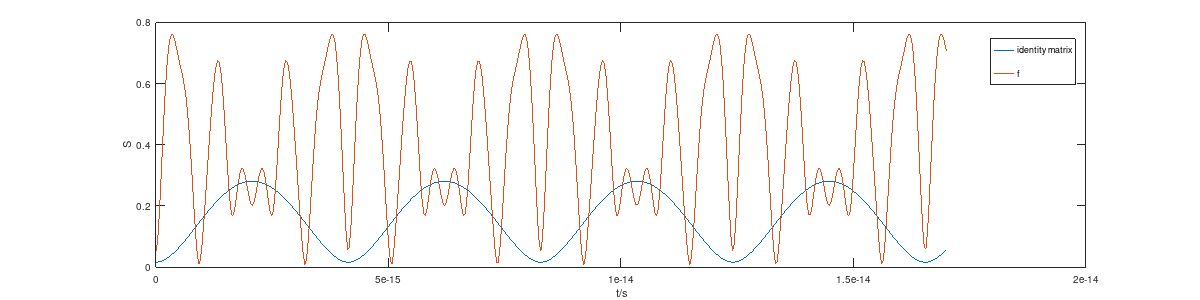
\includegraphics[width=19cm]{periodic_entropy.png}
  \caption{Periodische Entropie}
  \label{fig:periodic_entropy}
\end{center}\end{figure}

Abbildung \ref{fig:periodic_entropy} zeigt den Zeitverlauf der Entropie in der Teilung $f$. Er ist streng periodisch, da die Verhältnisse der Differenzfrequenzen rationale Zahlen sind. Die Periodendauer beträgt ca. 4,1 Femtosekunden.
Als Referenz wurde der Verlauf der Entropie in Originalsicht, d.h. mit der Einheitsmatrix als $f$, in die Grafik mit aufgenommen (blau).
\begin{figure}[!h]\begin{center}
  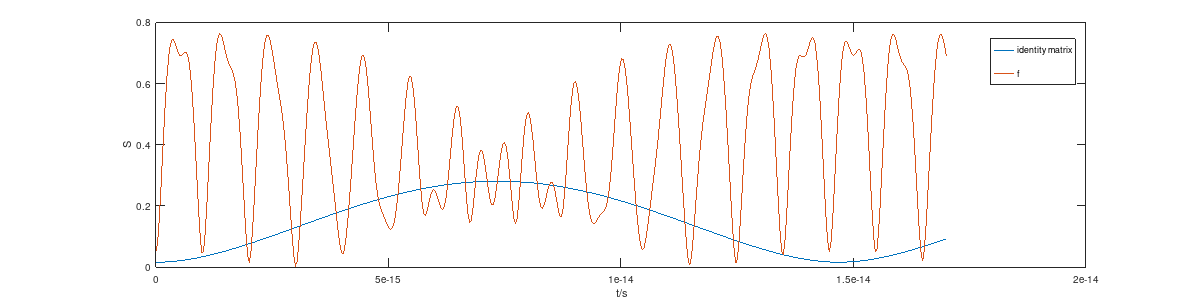
\includegraphics[width=19cm]{quasi_periodic_entropy.png}
  \caption{Quasiperiodische Entropie}
  \label{fig:quasi_periodic_entropy}
\end{center}\end{figure}

Wenn die Verhältnisse der Differenzfrequenzen nicht mehr alle rationale Zahlen sind, dann wird der Zeitverlauf quasiperiodisch. Für Abbildung \ref{fig:quasi_periodic_entropy} wurde der Energieeigenwert $7$ durch $2,6 \cdot e$ ersetzt.

\newpage
\section{Anhang D: Gnu Octave Programm}
Mit diesem Programm wurden die Zahlenbeispiele für diesen Artikel berechnet.
\begin{verbatim}
alpha_0=pi/6;
alpha_1=pi/5;

a_0_abs=sin(alpha_0+alpha_1)/sin(alpha_1-2*alpha_0)
a_1_abs=sin(alpha_0+alpha_1)/sin(alpha_0-2*alpha_1)
a_2_abs=1

a_0=a_0_abs*e^(i*alpha_0);
a_1=a_1_abs*e^(i*alpha_1);
a_2=a_2_abs;

% normalization
N=1/sqrt(a_0_abs^2+a_1_abs^2+a_2_abs^2);

% normalized orthogonal row vectors
u_0=[a_0,a_2,a_1]*N;
u_1=[a_1,a_0,a_2]*N;
u_2=[a_2,a_1,a_0]*N;

% check normalization
u_abs_square=u_0*u_0'

% check orthogonality
u_0_u_1=u_0*u_1'
u_1_u_2=u_1*u_2'
u_2_u_3=u_2*u_0'

% unitary matrix
U=[
u_0;
u_1;
u_2;
]

% null matrix
Null=U-U

% unistochastic matrix
P=[
[Null,U'.*conj(U')];
[U.*conj(U),Null];
]

% one clock tick
P_square=P*P

% external initial states
psi_0=[1,0,0,0,0,0]';
psi_1=[0,1,0,0,0,0]';
psi_2=[0,0,1,0,0,0]';

% time eigenvalues
t=[0,1,2,0,0,0];

% expectation values
exp_t_0 = t*P_square*psi_0
exp_t_1 = t*P_square*psi_1
exp_t_2 = t*P_square*psi_2

% entropy increase with clock ticks
p_1_tick=P_square*psi_0
p_2_ticks=P_square^2*psi_0
p_3_ticks=P_square^3*psi_0
\end{verbatim}

\end{document}
